\documentclass{beamer}
\usepackage[utf8]{inputenc} % Кодировка utf8
\usepackage[english, russian]{babel} % Языки: русский, английский
\usepackage{textcase}
\usepackage{geometry}
\usepackage{amsmath}
\usepackage{algorithm}
\usepackage{MnSymbol}
\usepackage{listings}
\usepackage{hyperref}
\usepackage{graphicx}
\usepackage{epstopdf}
\usetheme{Warsaw}
\usecolortheme{beaver}

\title[XS-схемы] % (optional, only for long titles)
{AS-схемы построения тактовых подстановок блочных криптосистем: характеристики перемешивания}
\author[Миронович С.] % (optional, for multiple authors)
{Миронович Светлана\\ 5 курс 9 группа, кафедра ММАД\\~ \\Руководитель: Агиевич Сергей Валерьевич \\ Заведующий НИЛ ПБИТ\\ кандидат физико-математических наук}
\institute[БГУ] % (optional)
{
  Белорусский государственный университет\\
  Факультет прикладной математики и информатики
}
\date[2017] % (optional)
{Минск, 2017}
\subject{Computer Science}

\begin{document}
\frame{\titlepage}
\begin{frame}
\frametitle{Схемы тактовых подстановок}
\begin{center}
Схема тактовой подстановки:

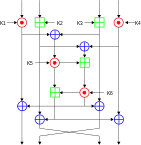
\includegraphics{2}
\end{center}
Допустимые операции: \{X, A, S, R, L, M\}.

Устойчивые сочетания: XS, LRX, ARX.
\end{frame}
  \begin{frame}
    \frametitle{$XS$ схемы}
В $XS$-схемах возможны только 2 операции:
\begin{itemize}
\item Операция исключающее ИЛИ
\item Подстановка в S-блок
\end{itemize}
$XS_1$-схемы - это схемы, где используется только один $S$-блок.
Все $XS_1$-схемы можно задать тройкой $(a, B, c)$ или расширенной матрицей:
$$
\begin{pmatrix}
b_{11} & b_{12} & \ldots & b_{1n} & a_1\\
b_{21} & b_{22} & \ldots & b_{2n} & a_2\\
\dotfill\\
b_{n1} & b_{n2} & \ldots & b_{nn} & a_n\\
c_1    & c_2    & \ldots & c_n    & 0\\
\end{pmatrix}.
$$
Тогда преобразование выглядит следующим образом:
$$Y = XB + S(Xa)c, X = (X_1, X_2, X_3, ..., X_n), Y = (Y_1, Y_2, Y_3, ..., Y_n)$$.
  \end{frame}

 \begin{frame}
    \frametitle{Подходы к изучению характеристик перемешивания на XS схемах}

\begin{itemize}
\item Граф и матрица зависимости

Граф зависимости - это граф, чьи вешины - это номера битов. Из $i$ есть ребро в $j$, если $i$-тый входной бит влияет на $j$-тый выходной (а вес ребра характеризует степень влияния).
\item Графы линейных и разностных переходов

Графы линейных и разностных переходов неявно описывают подверженность тактовой подстановки линейной и разностной атакам.
\end{itemize}
  \end{frame}

 \begin{frame}
    \frametitle{Граф и матрица зависимости}

Все преобразование зашифрования представим в виде подстановки $\sigma$.
Подстановке $\sigma$, действующей на $\{0,1\}^n$, 
поставим в соответствие {\it матрицу зависимостей}~$A_\sigma=(a_{ij})$.
Элемент $a_{ij}$ этой матрицы характеризует влияние $i$-го
бита прообраза~$\sigma$ на $j$-й бит образа.

Степень влияния можно описывать по-разному.
Рассмотрим два варианта:
\begin{enumerate}
\item
{\it Индикаторы}: $a_{ij}=1$,
если изменение $i$-го бита $X$ может привести 
к изменению $j$-го бита $\sigma(X)$,
и $a_{ij}=0$ в противном случае.

\item
{\it Вероятности}: 
$$
a_{ij}=\Pr\big\{\sigma(X)_j\neq \sigma(X\oplus 2^i)_j\colon
X\stackrel{R}\leftarrow\{0,1\}^n\big\}.
$$
\end{enumerate}
  \end{frame}

\begin{frame}
    \frametitle{Характеристики на матрице зависимости}

$\lambda_1, \lambda_2, ..., \lambda_n$, что $|\lambda_1| \ge |\lambda_2| \ge ... \ge |\lambda_n|$ - собственные значения матрицы зависимости.

Характеристики на матрице зависимости:

\begin{itemize}
\item Экспонент, $exp(G)$

Это степень, в которую нужно возвести матрицу зависимости, чтобы в ней не осталось нулей
\item $\lambda(G)$

Максимальное по модулю собственное значение, т.е. $\lambda_1$.
\item $k(G)$

$k(G) = \frac{\lambda_2}{\lambda_1}$
\end{itemize}

  \end{frame}

\begin{frame}
    \frametitle{Вычисления характеристик на криптосистеме belt}

Были вычислены характеристики $k(G), \lambda(G), exp(G)$ для вероятностной и индикаторной матрицы зависимости криптосистемы $belt$. Результаты следующие.

Индикаторная матрица зависимости:

$$k(G) = 0.13326654881663205$$
$$\lambda(G) = 109.7691521877077$$
$$exp(G) = 2$$

Вероятностная матрица зависимости:

$$k(G) = 0.3914373414043516$$
$$\lambda(G) = 1027.8610668901583$$
$$exp(G) = 2$$
  \end{frame}


\begin{frame}
    \frametitle{XS схемы и экспонент}
Как меняются характеристики при увеличении размера фрагмента в тактовой подстановке?

\textbf{Теорема:} Экспонент матрицы зависимости любой тактовой подстановки из класса XS не зависит от длины фрагмента $m$ для $m \ge 2$.

  \end{frame}

  \begin{frame}
    \frametitle{Графы линейных и разностных переходов}
Пусть у нас есть $XS_1$ схема, которая разбивает входное слово на $n$ частей.  

Основная цель построения графа линейных и разностных переходов - это научиться находить слабые места в тактовой подстановке с точки зрения некоторой атаки (соответственно, граф линейных переходов отражает слабости с точки зрения линейного криптоанализа; граф разностных переходов иллюстрирует подверженные разностной атаке места).
Данные графы имеют $2^n$ вершин и ориентированные ребра, которым присвоен вес либо 0, либо 1. Вес 0 означает уязвимый для соответствующей атаки переход в тактовой подстановке, вес 1 является желательным для ребер в данных графах.
  \end{frame}
\begin{frame}
 \frametitle{Характеристики на графах линейных и разностных переходов}
На графах линейных и разностных переходов можно ввести следующие характеристики:
\begin{itemize}
\item Легчайший маршрут заданной длины в графе.
Данная метрика отражает самую слабую последовательность переходов заданной длины в тактовой подстановке.
\item Цикл минимального среднего веса в графе (minimum cycle mean, mcm).
Данная метрика отражает подверженность атаке самой  слабой последовательности переходов в тактовой подстановке.
\end{itemize}
\end{frame}
\begin{frame}
\frametitle{Алгоритмы вычисления характеристик на графах линейных и разностных переходов}
Легчайший путь длины k:
\begin{itemize}
\item Модификация алгоритма Форда-Беллмана
\item Доказана корректность
\item Асимптотическая сложность: $O(mk)$, где $m$ - количество ребер, $k$ - длина маршрута.
\end{itemize}
Цикл минимального среднего веса:
\begin{itemize}
\item Модификация алгоритма нахождения легчайшего пути заданной длины
\item Асимптотическая сложность: $O(mn)$, где $n$ - количество вершин в графе, $m$ - количество ребер
\item Асимптотическая сложность наилучшего из найденных аналогов: $O(mn\log(n))$
\end{itemize}
\end{frame}
\begin{frame}
    \frametitle{Результаты вычисления mcm на графах линейных и разностных переходов}

\begin{tabular}{ l | c | c }
  \hline			
  Схема & mcm на графе & mcm на графе \\
   & разностных переходов & линейных переходов \\
\hline
  Feistel & 0.(6) & 0.(6) \\
  Skipjack A & 0.5(3) & 0.5(3) \\
  Skipjack B & 0.5(3) & 0.5(3) \\
  SMS4 & 0.(857142) & 0.4 \\
  Lai-Massey & 1& 1 \\
  Matsui-L & 0.5 & 0.5 \\
  Matsui-R & 0.(6) & 0.(6) \\
  GFN-1 & 0.5(3) & 0.5(3) \\
  GFN-1-Inv & 0.5(3) & 0.5(3)  \\
  MARS-3 & 0.4 & 0 \\
  \hline  
\end{tabular}

  \end{frame}
\begin{frame}
\frametitle{belt-keywrap}
\begin{itemize}
\item Один из алгоритмов СТБ 34.101.31
\item Используется для одновременного шифрования и контроля целостности данных
\item Масштабируем по количеству фрагментов. Приведем пример для количества фрагментов 3 и 4:

$$
\begin{pmatrix}
0 & 1 & 0 & 1\\
0 & 0 & 1 & 1\\
0 & 0  & 1 & 1\\
1 & 1 & 0 & 0\\
\end{pmatrix}, 
\begin{pmatrix}
0 & 1 & 0 & 0 & 1\\
0 & 0 & 1 & 0 & 1\\
0 & 0 & 0 & 1 & 1\\
0 & 0 & 0 & 1 & 1\\
1 & 1 & 0 & 0 & 0\\
\end{pmatrix}.
$$


\end{itemize}
\end{frame}
\begin{frame}
    \frametitle{Вычисление mcm на belt keywrap}

\begin{tabular}{ l | c | c }
  \hline			
  Длина блока & mcm на графе & mcm на графе \\
   & разностных переходов & линейных переходов \\
\hline
  2 & 0.(6) & 0.(6) \\
  3  & 0.75 & 0.5 \\
  4  & 0.8 & 0.(3) \\
  5 & 0.8(3) & 0.25 \\
  6 & 0.(857142) & 0.2 \\
  7 & 0.875 & 0.1(6) \\
  8 & 0.(8) & 0.(142857) \\
  9 & 0.9 & 0.125 \\
  10 & 0.(90) & 0.(1)  \\
  11 & 0.91(6) & 0.1 \\
  \hline  
\end{tabular}
Здесь прослеживается зависимость с длиной блока. Так, mcm для графа разностных переходов описывается формулой $\frac{n}{n+1},$ где $n$ - длина блока. Также mcm для графа линейных переходов может быть описан формулой $\frac{1}{n-1},$ где $n$ также длина блока.

  \end{frame}
\begin{frame}
\frametitle{Заключение}
В дипломной работе были получены следующие результаты:
\begin{itemize}
\item Разработан алгоритм построения матрицы зависимости.
\item Предложены и реализованы программно метрики на матрице зависимости.
\item Предложены и поддержаны программно алгоритмы построения графов линейных и разностных переходов.
\item Разработаны эффективные алгоритмы вычисления метрик на графах линейных и разностных переходов.
\item Проведены вычислительные эксперименты на некоторых известных тактовых подстановках при помощи разработанного ПО.
\end{itemize}

Весь реализованный код находится в открытом доступе и может быть найден по ссылке: \url{https://github.com/mazukta26/Diploma}.
\end{frame}

\begin{frame}
\begin{center} \textbf{Спасибо за внимание!} \end{center}
\end{frame}
% etc
\end{document}